% !TEX root = deckblatt3b.tex

\section{Invertierender Verst\"arker}
\subsection{Aufgabenstellung}
Es soll ein invertierender OPV aufgebaut werden und desen Funktion durch Stom- und Spannungsmessung gepr\"uft werden. Anschlie\ss{}end soll das Frequnezverhalten des OPVs mithilfe von Bodediagrammen festgehalten werden.

\subsection{Schaltung}

\begin{figure}[H]
  \begin{center}
    %\tikzset{component/.style={draw,thick,circle,fill=white,minimum size =0.75cm,inner sep=0pt}}
    \begin{circuitikz}
    \draw
    (-2,2) node[ground] (ground) {}
    (3,4) node[op amp] (opamp) {}
    (3,4.5) to[short] (3,5) node[vcc] {$V_{CC}$}
    (3,3.5) to[short] (3,3) node[vss] {$V_{SS}$}
    (opamp.-) to[R={$R_1$}{$=1,5k$}] (-2,4.5)
    (opamp.+) to[short] (1.5,3.5) to[short] (1.5,2) node[ground] (ground) {}
    (1.5,4.5) to[short] (1.5,6.5) to[R={$R_2$}{$=82k$}] (4.5,6.5) to[short] (4.5,4)
    (opamp.out) to[short] (6,4)
    (6,2) node[ground] (ground) {}
    ;
    \draw (-2,4.2) to[short] (-2,2.7) node[vee] {};
    \draw (-1.5,3) node[] {$U_e$};
    \draw (6,3.7) to[short] (6,2.7) node[vee] {};
    \draw (6.5,3) node[] {$U_a$};
    \end{circuitikz}
    \caption{nicht inververtierender OPV}
  \end{center}
\end{figure}
\noindent
Da es sich bei dieser Schlatung um einen invertierenden Verst\"arker handelt, wird die Eingangsspannung an den invertierenden Eingang des OPV geschaltet.
Der Ausgang wird ebenfalls auf den invertierenden Eingang gegengekoppelt, um eine brauchbare Verst\"arkung einstellen zu k\"onnen. Ein Idealer OPV ohne Gegenkopplung w\"urde die Differenzspannung zwischen invertierenden und nicht-invertierenden Eingang $\infty$ verst\"arken. Die Verst\"arkung wird mit den beiden Widerst\"anden $R_1$
und $R_2$ eingestellt. Die beiden Spannungsquellen $V_2$ und $V_3$ stellen die symmetrische Versorgungsspannung von $-15V$ bis $+15V$ dar.\\ \\
$\frac{U_e}{U_a}=-\frac{R_1}{R_2} \Rightarrow U_a=-U_e*\frac{R_2}{R_1} \Rightarrow V=-\frac{R_2}{R_1}$ \\ \\
Da sich die Verst\"arkung $V$ laut Angabe zwischen $-40$ und $-60$ befinden soll wurden f\"ur die Widerst\"ande folgende Werte gew\"ahlt: \\ \\
$R_1=82k\Omega$ \\
$R_2=1,5k\Omega$ \\
$V=-\frac{82k \Omega}{1,5k\Omega}=-54,7$

\subsection{Strom- und Spannungsmessung}
\begin{table}[H]
\begin{minipage}{.5\textwidth}
\begin{figure}[H]
\centering
 \begin{tabular}{c|c}
  $U_e$ & $96,4mV$ \\ \hline
  $U_a$ & $-5,2V$ \\ \hline
  $U_{R1}$ & $95,6mV$ \\ \hline
  $U_{R2}$ & $-5,15V$ \\ \hline
  $U_d$ & $-0,4mV$ \\ \hline
  $I_{R1}$ & $63\mu A$ \\ \hline
  $I_{R2}$ & $63\mu A$ \\ \hline
  $I_+$ & $0mA$ \\ \hline
  $I_-$ & $0mA$ \\
 \end{tabular}
  \caption{Messwerte $0,1V$ DC}
\end{figure}
\end{minipage}
\begin{minipage}{.5\textwidth}
\begin{figure}[H]
  \centering
 \begin{tabular}{c|c}
  $U_e$ & $309,1mV$ \\ \hline
  $U_a$ & $-13,6V$ \\ \hline
  $U_{R1}$ & $265,2mV$ \\ \hline
  $U_{R2}$ & $-14,39V$ \\ \hline
  $U_d$ & $-575mV$ \\ \hline
  $I_{R1}$ & $169\mu A$ \\ \hline
  $I_{R2}$ & $169\mu A$ \\ \hline
  $I_+$ & $0mA$ \\ \hline
  $I_-$ & $0mA$ \\
 \end{tabular}
 \caption{Messwerte $0,3V$ DC}
\end{figure}
\end{minipage}
\end{table}
\noindent
Die Strom- und Spannungsmessungen wruden mit zwei verschiedenen Eingangsspannungen durchgef\"uhrt, einmal mit $100mV$ Gleichspannung und einmal mit $300mV$ Gleichspannung. Die Messungen passen sehr gut mit den Simulationsergebnissen \"uberein. \\
Man kann in den Messungen die Verst\"arkung lt. Messung betr\"agt $V=\frac{-5.2}{0.0964}=-53,9$ Dieser Wert passt mit der errechneten Verst\"arkung von $V=-54,7$ sehr gut \"uberein. Die Str\"ome welche an den Eing\"angen in den OPV flie\ss{} waren zu klein um sie mit dem Ampermeter messen zu k\"onnen, dies stimmt mit der Theorie sehr gut \"uberein da bei einem idealen OPV auf Grund des unendlich großen Eingangswiderstandes kein Strom hineinflie\ss{}en kann. Der Srom durch die Beiden Widerst\"ande ist ebenfalls wie erwartet der gleiche.

\subsection{Messungen im Zeitbereich}
\begin{figure}[H]
 \begin{center}
  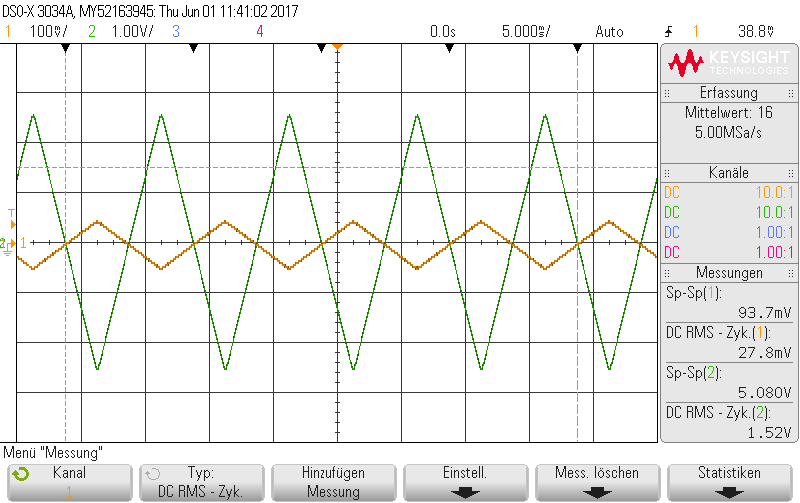
\includegraphics[height=6cm,width=12cm]{OsziBilder/InvVer_100Hz}
 \end{center}
 \caption{Dreieckspannung $0,1V_{pp}$, $100Hz$ ($U_e$ orange, $U_a$ grün)}
\end{figure}

\begin{figure}[H]
 \begin{center}
  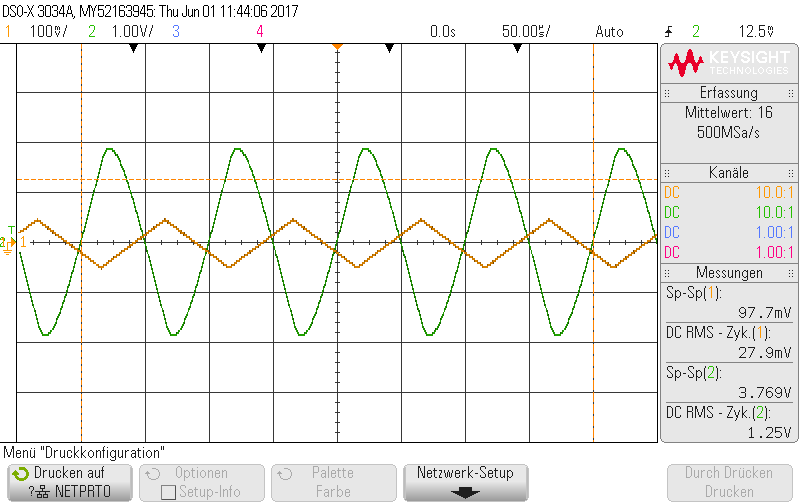
\includegraphics[height=6cm,width=12cm]{OsziBilder/InvVer_10kHz}
 \end{center}
 \caption{Dreieckspannung $0,1V_{pp}$, $10kHz$ ($U_e$ orange, $U_a$ grün)}
\end{figure}
\noindent
Das $100Hz$ Signal zeigt eine schöne invertierte $1:48$ Übertragung. Bei $10kHz$ jedoch
wurde die Grenzfrequenz der Operationsverstärkerschaltung überschritten und das bauteilbedingte
Tiefpassverhalten wirkt sich aus. So wird das Signal nicht mehr korrekt Verstärkt und verschliffen übertragen.\\
\newpage


\subsection{Bodediagramm}
Es sollten zwei Bodediagramme aufgenommen werden, f\"ur beide wurde eine Sinusspannung mit $100mVpp$ als Eingnagssingal gew\"ahlt. Bei der zweiten Messung wurde die Verst\"arkung um den Fatkor 10 veringert, dies wurde durch eine Verringerung des Widerstandes $R_2$ von $82k\Omega$ auf $8,2k\Omega$ bewerkstelligt.

\begin{figure}[H]
  \centering
  \begin{tikzpicture}
    \begin{axis}[width=15cm, height=7cm, xmode=log, xmin=10, xmax=1e6, xlabel={Frequenz [Hz]}, ylabel={Amplitude [dB]},y tick label style={grid=major}]
      \addplot table[x=Frequenz, y=dB, col sep=comma] {./csv_files/invVer_bigAmpl.csv};
      %\node[label={260:{$f_g$}},circle,fill=black,inner sep=3pt] at (axis cs:15580,12) {};
    \end{axis}
  \end{tikzpicture}
  \caption{invertierender Verst\"arker, $V=-54,7$, Amplitudengang}
\end{figure}
\begin{figure}[H]
  \centering
  \begin{tikzpicture}
    \begin{axis}[width=15cm, height=7cm, xmode=log, xmin=10, xmax=1e6, xlabel={Frequenz [Hz]}, ylabel={Phase [$^\circ$]},y tick label style={grid=major}]
      \addplot table[x=Frequenz, y=Phi, col sep=comma] {./csv_files/invVer_bigAmpl.csv};
      %\node[label={260:{$f_g$}},circle,fill=black,inner sep=3pt] at (axis cs:15580,12) {};
    \end{axis}
  \end{tikzpicture}
  \caption{invertierender Verst\"arker, $V=-54,7$, Phasengang}
\end{figure}
\noindent
In diesem Bodediagramm ist sehr gut die Transitfrequnezn von $1MHz$ zu erkennen. Da sich ein realer OPV intern wie ein Tiefpassfilter verh\"alt nimmt die Verst\"arkung von der Grenzfrequnez bis zur Transitfrequnez mit $-20dB/DEK$ ab. Eine Verst\"arkung von $-54,7$ entspricht $34,76dB$ d.h. die D\"ampfung wird bei dieser Beschaltung erst ab $10kHz$ bemerkbar.

\begin{figure}[H]
  \centering
  \begin{tikzpicture}
    \begin{axis}[width=15cm, height=7cm, xmode=log, xmin=10, xmax=1e6, xlabel={Frequenz [Hz]}, ylabel={Amplitude [dB]},y tick label style={grid=major}]
      \addplot table[x=Frequenz, y=dB, col sep=comma] {./csv_files/invVer_smlAmpl.csv};
      %\node[label={260:{$f_g$}},circle,fill=black,inner sep=3pt] at (axis cs:15580,12) {};
    \end{axis}
  \end{tikzpicture}
  \caption{invertierender Verst\"arker, $V=-5,47$, Amplitudengang}
\end{figure}
\begin{figure}[H]
  \centering
  \begin{tikzpicture}
    \begin{axis}[width=15cm, height=7cm, xmode=log, xmin=10, xmax=1e6, xlabel={Frequenz [Hz]}, ylabel={Phase [$^\circ$]},y tick label style={grid=major}]
      \addplot table[x=Frequenz, y=Phi, col sep=comma] {./csv_files/invVer_smlAmpl.csv};
      %\node[label={260:{$f_g$}},circle,fill=black,inner sep=3pt] at (axis cs:15580,12) {};
    \end{axis}
  \end{tikzpicture}
  \caption{invertierender Verst\"arker, $V=-5,47$, Phasengang}
\end{figure}
\noindent
F\"ur diese Messung wurde wie oben bereits beschrieben die Verst\"arkung um den Faktor 10 verringert. Da nun de Ferst\"arkung um den Faktor 10 kleiner ist macht sich auch die D\"ampfung des OPVs erst eine Dekade sp\"ater bemerkbar, ab dann f\"alls sie jedoch genauso mit -20dB/Dek ab.
\newpage
